\chapter{Transformer and Shunt Reactor}
\label{chap:transformer-shunt-reactor}
\index{transformer}
\index{shunt reactor}

\section{General}
\label{sec:tsr-general}

In the first example, a three-phase circuit is examined. The case of an inductive load, namely the switching-on of a shunt reactor, and its impact on the voltage are investigated. The load is energized first by one transformer and then by two transformers. Finally, a special case with two transformers in series is presented. Such a configuration can occur when a de-energized part of a network is restored from a network section that is already energized (for instance after a blackout).


\section{Circuit Design}
\label{sec:tsr-circuit-design}
The example file \texttt{Transformer\_and\_shunt\_reactor.asc} is for the first transient (.TRAN) analysis. 
Additional measurements defined with \texttt{.meas} in the LTspice schematic are written to the \texttt{spice-output-logfile} file at the end of the simulation. In LTspice, this file can be opened with \emph{View~$\rightarrow$~SPICE Output Log}. 
To set simulation accuracy for voltages and currents the LTspice netlist settings are:\\ 

\begin{lstlisting}[style=LTspice]
	.options vntol=1m
	.options abstol=1u
\end{lstlisting}

\noindent These values are much higher as at normal LTspice simulations with electronic circuits.

\begin{remark}{Convergence}{Remark11}
	If you encounter convergence problems you can try to increase \texttt{vntol} and \texttt{abstol}.
	You can also try to set the relative tolerance \texttt{reltol} to 0.01
	Changing the default integration mode can also be helpful.
\end{remark}

\noindent The following line for frequency and angular velocity should be included in every schematic:\\

\begin{lstlisting}[style=LTspice]
	.param tdv=1 tdt=1 fn1=50Hz(60Hz) omega_n={2*pi*fn1}
\end{lstlisting}

\noindent tdv=1 and tdt=1 are LTspice parameters used to avoid convergence problems with electrical power networks.
This first example contains buses, an impedance, transformers, and shunt reactors. The bus elements provide external measurement pins and the setting for the line-to-line voltage. Elements with three pins, such as \texttt{bus\_v}, measure all three line-to-line voltages as instantaneous values (bus\_v) or RMS values (bus\_Veff). During simulation the RMS values require some time to settle.

For modeling the net-impedance the model impedance\_sk is used. The model use nominal voltage and short-circuit power as inputs, assuming equal values for all phases. The values for SN and UN should be:\\
\newpage

\begin{lstlisting}[style=LTspice]
SN=40e9
UN=400k
\end{lstlisting}

The transformer model used in this circuit is a simple linear model without a magnetic core, because a nonlinear core is not required for this example. After placing the symbol \texttt{trafo\_yy}, the model \texttt{RUYy0\_400k\_120k\_300MVA\_simple} is selected in the SpiceModel field (double-click to open the drop-down list) in the attribute editor. Other default parameter lines are removed.\\

The three-phase voltage source is started with exponential damping using the parameter \texttt{Texp=50ms}. This accelerates the settling of the current of the shunt reactor. The shunt reactor has a rating of \SI{50}{\mega\varunit} and a nominal voltage of \SI{110}{\kilo\volt}. Its nominal current is approximately \SI{250}{\ampere} RMS. The total simulation time is set to \SI{4}{\second}.

\noindent This is set by the .tran command of LTspice

\begin{lstlisting}[style=LTspice]
.tran 0 4s 0m 0.1m
\end{lstlisting}
A value of 0.1m specifies a maximum time step of 0.1 ms, which should be sufficiently small to resolve 50 Hz or 60 Hz sinusoidal waveforms accurately. Use a smaller time step for higher frequencies. For the following four examples the ltspice file is 
\texttt{Transformer\_and\_shunt\_reactor.asc}

\subsection{Transformer Without Shunt Reactor}
\label{sec:without-shunt-reactor}

The voltage at the bus is approximately \SI{119.7}{\kilo\volt}. Thus, the nominal voltage of \SI{120}{\kilo\volt} is nearly reached. The small difference is caused by the series impedance of the network, which slightly reduces the voltage. 

\subsection{One Transformer and Shunt Reactor}
\label{sec:one-transformer-shunt-reactor}

In this case, the shunt reactor reduces the voltage to approximately \SI{115.1}{\kilo\volt}. The RMS current is approximate \SI{275}{\ampere}. This is higher than the rough estimate of \SI{250}{\ampere}, because the operating voltage is higher than the nominal voltage of the shunt reactor.

\subsection{Two Transformers in Parallel and Shunt Reactor}
\label{sec:parallel-transformers-shunt-reactor}

With two transformers connected in parallel, the equivalent internal impedance is reduced by a factor of two. Consequently, the voltage drop is smaller, and the voltage reaches approximately \SI{117.3}{\kilo\volt}. The current through the shunt reactor increases to approximately \SI{280}{\ampere} because of the higher operating voltage.

\subsection{Two Transformers in Series and Shunt Reactor}
\label{sec:series-transformers-shunt-reactor}

The shunt reactor is now supplied from a \SI{120}{\kilo\volt} source through two transformers connected in series. The transformer impedance is therefore doubled, and the voltage is reduced from \SI{119.2}{\kilo\volt} to approximately \SI{110.5}{\kilo\volt} corresponding to a voltage drop of \SI{8.7}{\kilo\volt}. The shunt-reactor current is approximately \SI{264}{\ampere}.
This configuration can arise when a de-energized part of a network is restored from a network section that remains energized (for instance after a blackout). Because of the large combined transformer impedance, the voltage is particularly sensitive to load changes in this configuration.

\subsection{Transformer and Shunt Reactor for AC-Analysis}
\noindent For an AC analysis the filename of the example is \texttt{Transformer\_and\_shunt\_reactor\_AC.asc}.
For the AC analysis, the voltage-source model is changed to \texttt{V\_3phase\_AC}. The transient-analysis directive \texttt{.tran} is replaced by an \texttt{.ac} directive. For measuring the bus voltages
the transient bus models must be replaced with the appropriate ac bus models \texttt{bus\_V} with \texttt{bus\_V\_AC} to measure line to line voltages and \texttt{bus\_Veff} with \texttt{bus\_V0\_AC} to measure line to earth voltages.

\begin{important}{AC-Analysis}{important11}
	Linear AC analysis linearizes nonlinear elements at the operating point and is therefore not suitable for large-signal analysis.
\end{important}

%\noindent On the next page Figure~\ref{fig:schematic1} shows the Schematic for the Transformer and shunt %reactor AC example and ..\\

%\noindent .. on the following page Figure~\ref{fig:Transformer_and_shunt_reactor_AC_Waveform} shows the %steady-state AC phase voltages together with the currents flowing through the shunt reactors.\\

%\begin{example}{Transformer and shuntreactor AC}{}
%	Shows the schematic and output of the waveformviewer for AC-Analysis
%\end{example}


%\vspace{0.1pt}

\section{Manual Calculation of the Line-to-Line Voltage Drop with Two Transformers in Series}
\label{sec:manual-calculation-series-case}

	The internal impedance of a \SI{400}{\kilo\volt}/\SI{120}{\kilo\volt} transformer is approximately \SI{9.6}{\ohm} inductive when referred to the secondary side. (See equation ~\ref{eq:eqn1_9}). For two transformers connected in series, the total impedance is therefore approximately

\begin{calculation}{Voltage reduction}{calculation11}

	\begin{align}
		X_{\mathrm{T,tot}} &= 2 \cdot \SI{9.6}{\ohm}
		= \SI{19.2}{\ohm}.
	\end{align}
	
	With a current of approximately \SI{264}{\ampere}, the phase-voltage drop is
	
	\begin{align}
		\Delta U_{\mathrm{ph}}
		&= I X_{\mathrm{T,tot}} \\
		&= \SI{264}{\ampere} \cdot \SI{19.2}{\ohm} \\
		&= \SI{5}{\kilo\volt}.
	\end{align}
	
	The corresponding line-to-line voltage drop is approximately
	
    \begin{align}
	\Delta U_{\mathrm{LL}}
	&= \sqrt{3}\,\Delta U_{\mathrm{ph}} \\
	&\approx 1.73 \cdot \SI{5}{\kilo\volt} \\
%	&\approx \SI{8.65}{\kilo\volt}.
    &\approx\boxed{\mathbf{\SI{8.65}{\kilo\volt}}}
    \end{align}
	
	This result agrees well with the simulated voltage reduction in \cref{sec:series-transformers-shunt-reactor}.\\
\end{calculation}



\noindent To get the value of the leakage impedance of transformer 
we can see the wxmaxima file \texttt{transformer\_400kV\_120kV\_yy.wxmx} and search for xkus.

\begin{calculation}{Leakage impedance}{calculation12}
    \begin{align}
	X_{1\mathrm{s}}
	&= L_{1\mathrm{s}}\,\omega \nonumber\\
	&= 0.1697 \cdot 314.159 \nonumber\\
	&= \SI{53.33}{\ohm} \\[2ex]
	X_{2\mathrm{s}}
	&= X_{1\mathrm{s}}
	\frac{(\SI{120}{\kilo\volt})^{2}}
	{(\SI{400}{\kilo\volt})^{2}}
	\nonumber\\
	&= \boxed{\mathbf{\SI{9.60}{\ohm}}} 
	\label{eq:eqn1_9}
%	&= \SI{9.60}{\ohm}
    \end{align}
\end{calculation}

\begin{figure}[H]
	\centering
    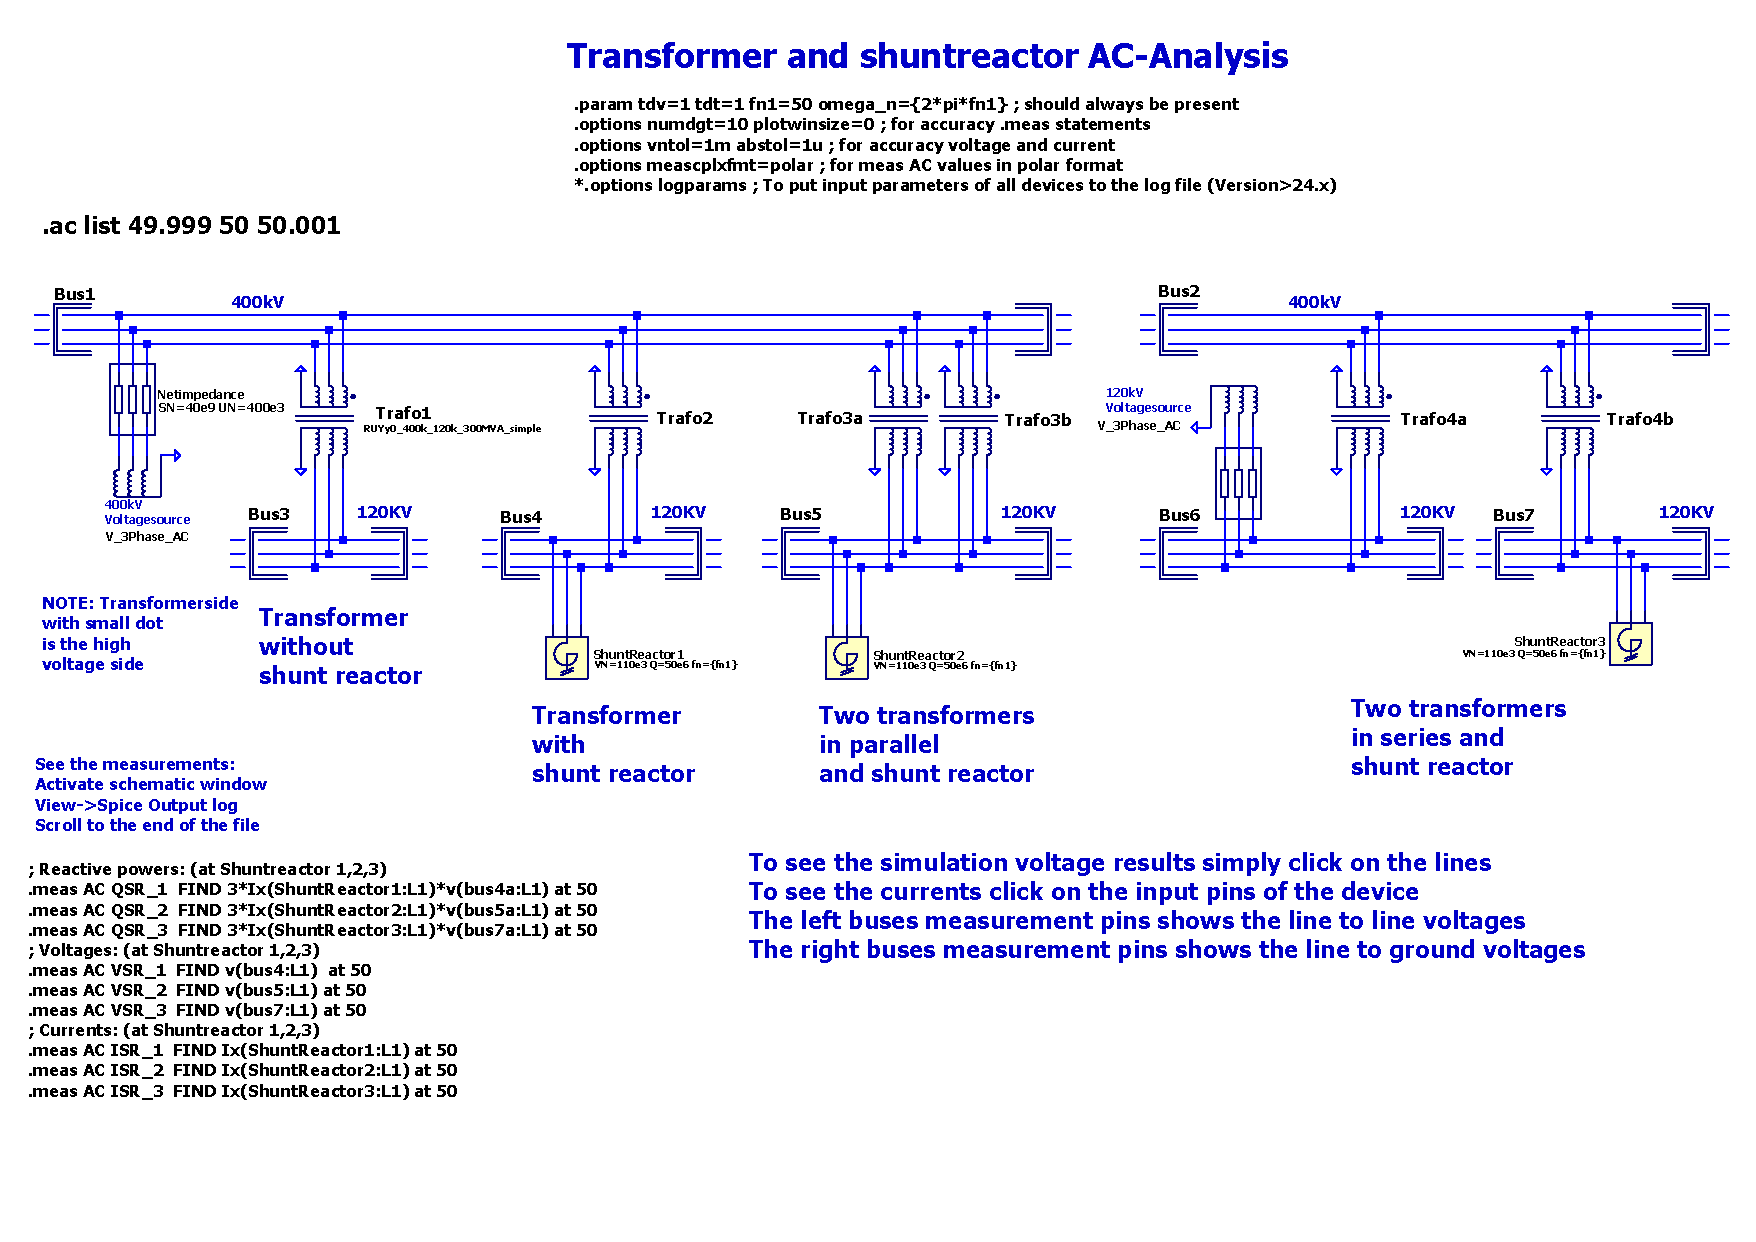
\includegraphics[width=1\textwidth]{figures/01_Transformer und shunt reactor/Transformer_and_shunt_reactor_AC_Schematic.pdf}
	\caption{AC voltages and currents at the shunt reactors.}
	\label{fig:Transformer_and_shunt_reactor_AC_Waveform}
\end{figure}

%\begin{figure}[H]
%	\centering
%	\includegraphics[width=0.99\textwidth]{figures/Transformer_and_shunt_reactor_AC_Schematic}
%	\caption{Schematic for the Transformer and shunt reactor circuit.}
%	\label{fig:Transformer_and_shunt_reactor_AC_Schematic}
%\end{figure}


\begin{figure}[H]
	\centering
	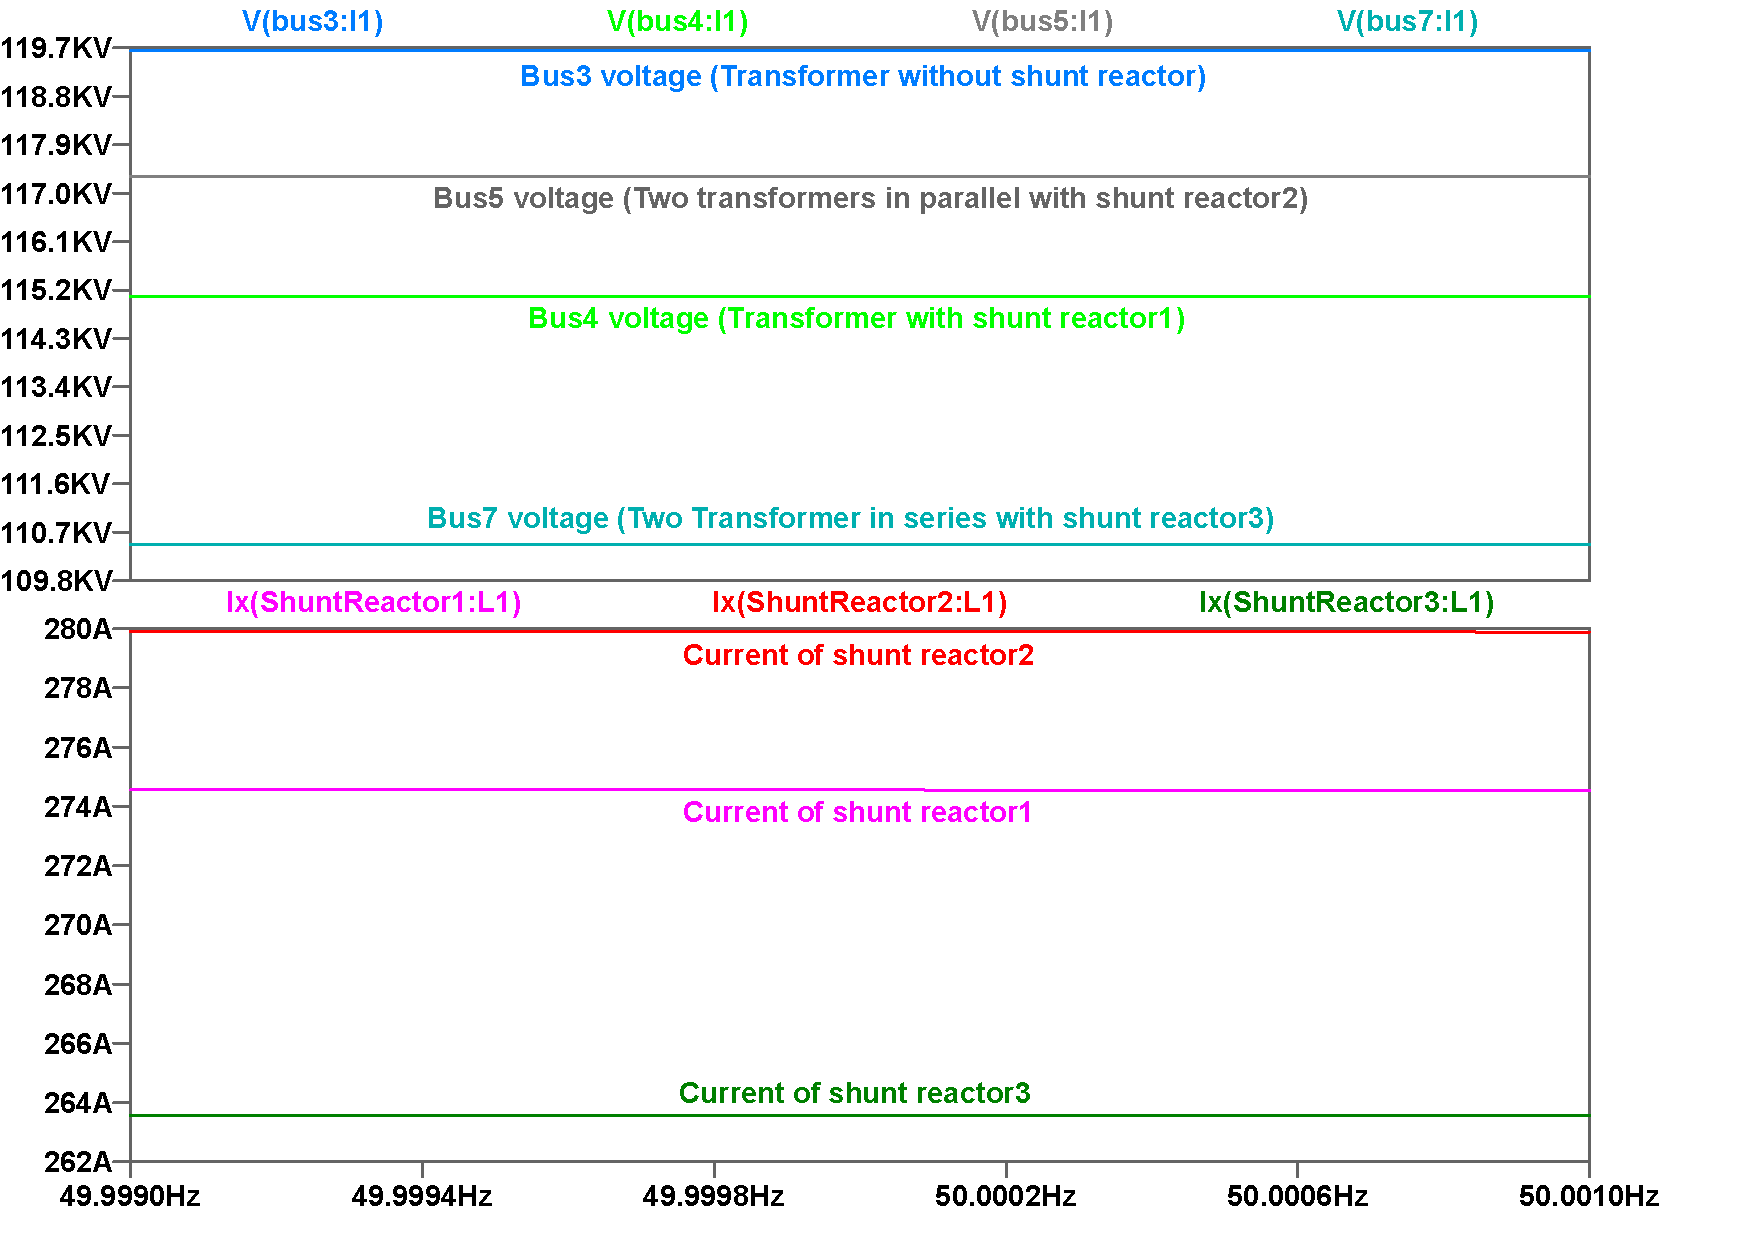
\includegraphics[width=0.90\textwidth]{figures/01_Transformer und shunt reactor/Transformer_and_shunt_reactor_AC_waveform}
	\caption{AC voltages and currents at the shunt reactors.}
	\label{fig:Transformer_and_shunt_reactor_AC_Waveform}
\end{figure}


\begin{chaptersummary}
Shunt reactors are used to regulate the voltage in a power grid. It operates as standalone device or are connected to the tertiary winding of a high voltage transformer.
In this chapter, we have seen that loading a circuit with a shunt reactor reduces the voltage towards the shunt reactor. This voltage reduction occurs whenever a current flow through transformers or the line impedance, which is also highly inductive. As a rule of thumb, inductive reactive power generally flows from the higher voltage level to the lower voltage level. When the transformer is loaded with pure active power, active power always flows from the higher voltage phase angle to the lower voltage angle. 
Real-world example: After energizing a network section via two transformers in series, the voltage is highly volatile. It is best to energize the power district with balanced reactive power. Voltage regulation in the power district should be performed using the regulating transformers and not the shunt reactor. 	
\end{chaptersummary}

